%---------------------------------------------------------------------
% Course 	: Introduction To web sciences
% Professor : Dr.Nelson
% Name   	: Babitha Bokka
% Assignment: 6
%---------------------------------------------------------------------
\documentclass[12pt]{article}
%--------------------------------------------------------------------
% packages required
%--------------------------------------------------------------------
\usepackage{graphicx}
\usepackage{listings}
\usepackage{hyperref}
\usepackage{caption}
\usepackage{color}
\usepackage{pdfpages}
\graphicspath{ {images/} }
%--------------------------------------------------------------------
% Start Margins
%--------------------------------------------------------------------
\addtolength{\oddsidemargin}{-.875in}
\addtolength{\evensidemargin}{-.875in}
\addtolength{\textwidth}{1.75in}
\addtolength{\topmargin}{-.885in}
\addtolength{\textheight}{1.95in}
%-------------------------------------------------------------------
% End Margins
%--------------------------------------------------------------------
\definecolor{codegreen}{rgb}{0,0.6,0}
\definecolor{codegray}{rgb}{0.5,0.5,0.5}
\definecolor{codepurple}{rgb}{0.58,0,0.82}
\definecolor{backcolour}{rgb}{0.95,0.95,0.92}
 
\lstdefinestyle{mystyle}{
    backgroundcolor=\color{backcolour},   
    commentstyle=\color{codegreen},
    keywordstyle=\color{magenta},
    numberstyle=\tiny\color{codegray},
    stringstyle=\color{codepurple},
    basicstyle=\footnotesize,
    breakatwhitespace=false,         
    breaklines=true,                 
    captionpos=b,                    
    keepspaces=true,                 
    numbers=left,                    
    numbersep=5pt,                  
    showspaces=false,                
    showstringspaces=false,
    showtabs=false,                  
    tabsize=2
}
 
\lstset{style=mystyle}

\begin{document}

%---------------------------------------------------------------------
%Making the title page
%---------------------------------------------------------------------
\begin{titlepage}
\title{INTRODUCTION TO WEB SCIENCES:\\*Assignment 6}
\author{Babitha Bokka}
\date{1 November 2014}
\maketitle
\end{titlepage}

%---------------------------------------------------------------------
%Table of contents
%---------------------------------------------------------------------
\tableofcontents
\newpage
%------------------------------------------------------------------
%Question 1
%------------------------------------------------------------------
\section{Question 1: Karate group split into 2 groups}
Prove or disprove the result of the split could have been predicted by the weighted graph of social interactions. How well the mathematical model would represent the reality.
%-----------------------Approach----------------------------------
\subsection{Approach}
karate club splits into two after the dispute. So, we now compute  a mathematical model using Girvan-Newman Algorithm which can split the groups into two by using the edge betweeness. In order to acheive this we take karate.GraphML file observe the node and edge weights. Based on the edge betweeness identify the edges to be removed. \\*
According to Girvan-Newman Algorithm karateClubGraph.py calculate the edge betweness, finds the edge with maximum betweeness and deletes the edge.

\subsection{Description of karateClubGraph.py}
\begin{enumerate}
	\item Load the karate.GraphML.
	\item Label all the nodes.
	\item Plot the graph to check how the graph is connected before the split.
	\item Calculate the betweeness of the all the edges in the graph.
	\item Find the edge with maximum betweeness.
	\item Remove the edge with maximum betweeness.
	\item Repeat the steps in a loop until the single cluster becomes two clusters.
	\item Plot the graph with clusters.
	\item Verify the output with the reality. You can manually draw the the graph for the karate.GraphML file and check whether the predicted graphs will represent the real graphs .	 
\end{enumerate}
 \newpage
%-----------------------Source Code-------------------------------
\subsection{Source Code}
\subsubsection{karateClubGraph.py}
\lstinputlisting[breaklines=True,language=Python]{../Q1/karateClubGraph.py}
\newpage
%-----------------------Input Section---------------------------
\subsection{Input}
\subsubsection{karate.GraphML}
\lstinputlisting[breaklines=True]{../Q1/karateGraphMLForDoc.txt}
\newpage

%-----------------------Output Section---------------------------
\subsection{Output Files}
Figure~\ref{fig:initial-graph} is the initial graph generated from the karate.GraphML. If we observe the graph each node is connected to some other nodes but there are strong and weekly connected edges. Now, we can split the graph manually and know which person is in support of whom. Figure~\ref{fig:Graph in split Reality 1}, Figure~\ref{fig:Graph in split Reality 2} represent the actual split of the group in reality.
Figure~\ref{fig:Graph after split} has two clusters formed by predicting the weighted graph.
\subsubsection{Intial Graph}
\begin{figure}[ht]
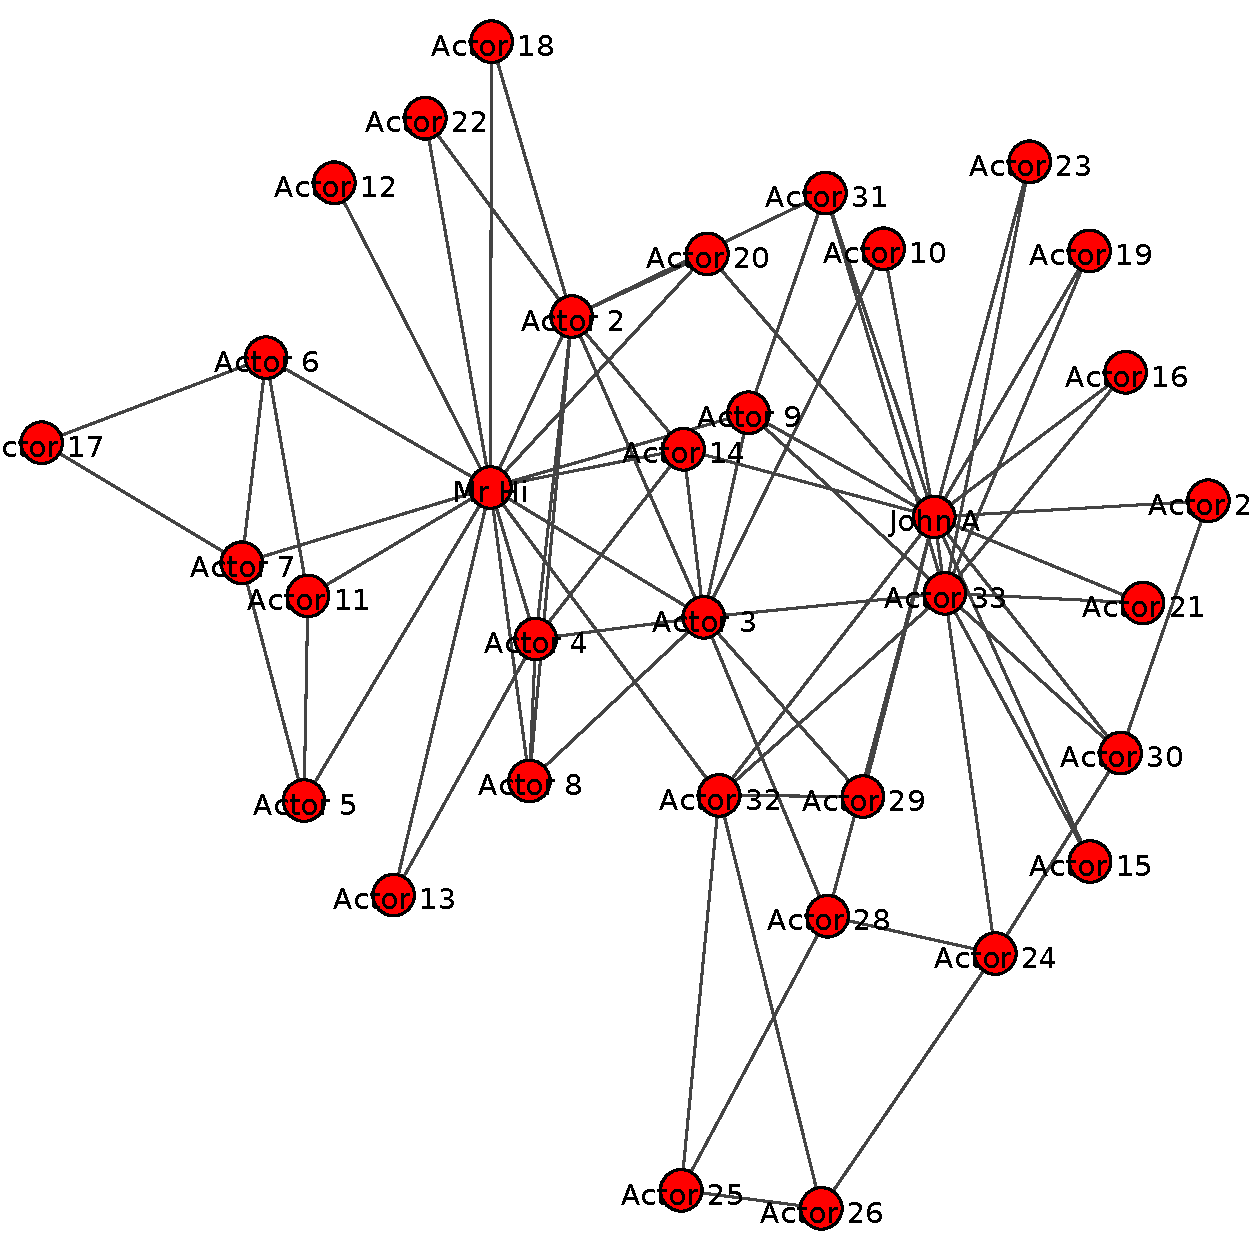
\includegraphics[scale=0.7]{../Q1/graph1.pdf}
\centering
\caption{initial-graph}
\label{fig:initial-graph}
\end{figure}
\newpage

\subsection{Graphs after the split}
\subsubsection{Graph split Reality}
\begin{figure}[ht]
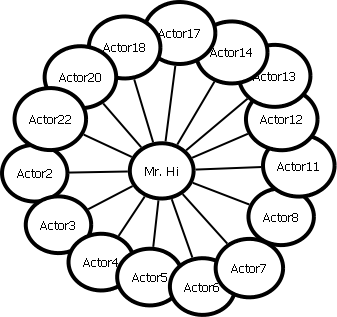
\includegraphics[scale=0.7]{../reality1}
\centering
\caption{Reality 1}
\label{fig:Graph in split Reality 1}
\end{figure}
\newpage
\begin{figure}[ht]
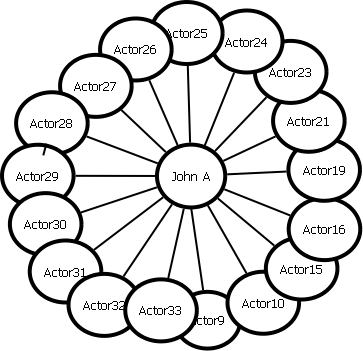
\includegraphics[scale=0.7]{../reality2}
\centering
\caption{Reality 2}
\label{fig:Graph in split Reality 2}
\end{figure}
\newpage

\subsubsection{Predicted graph after split}
\begin{figure}[ht]
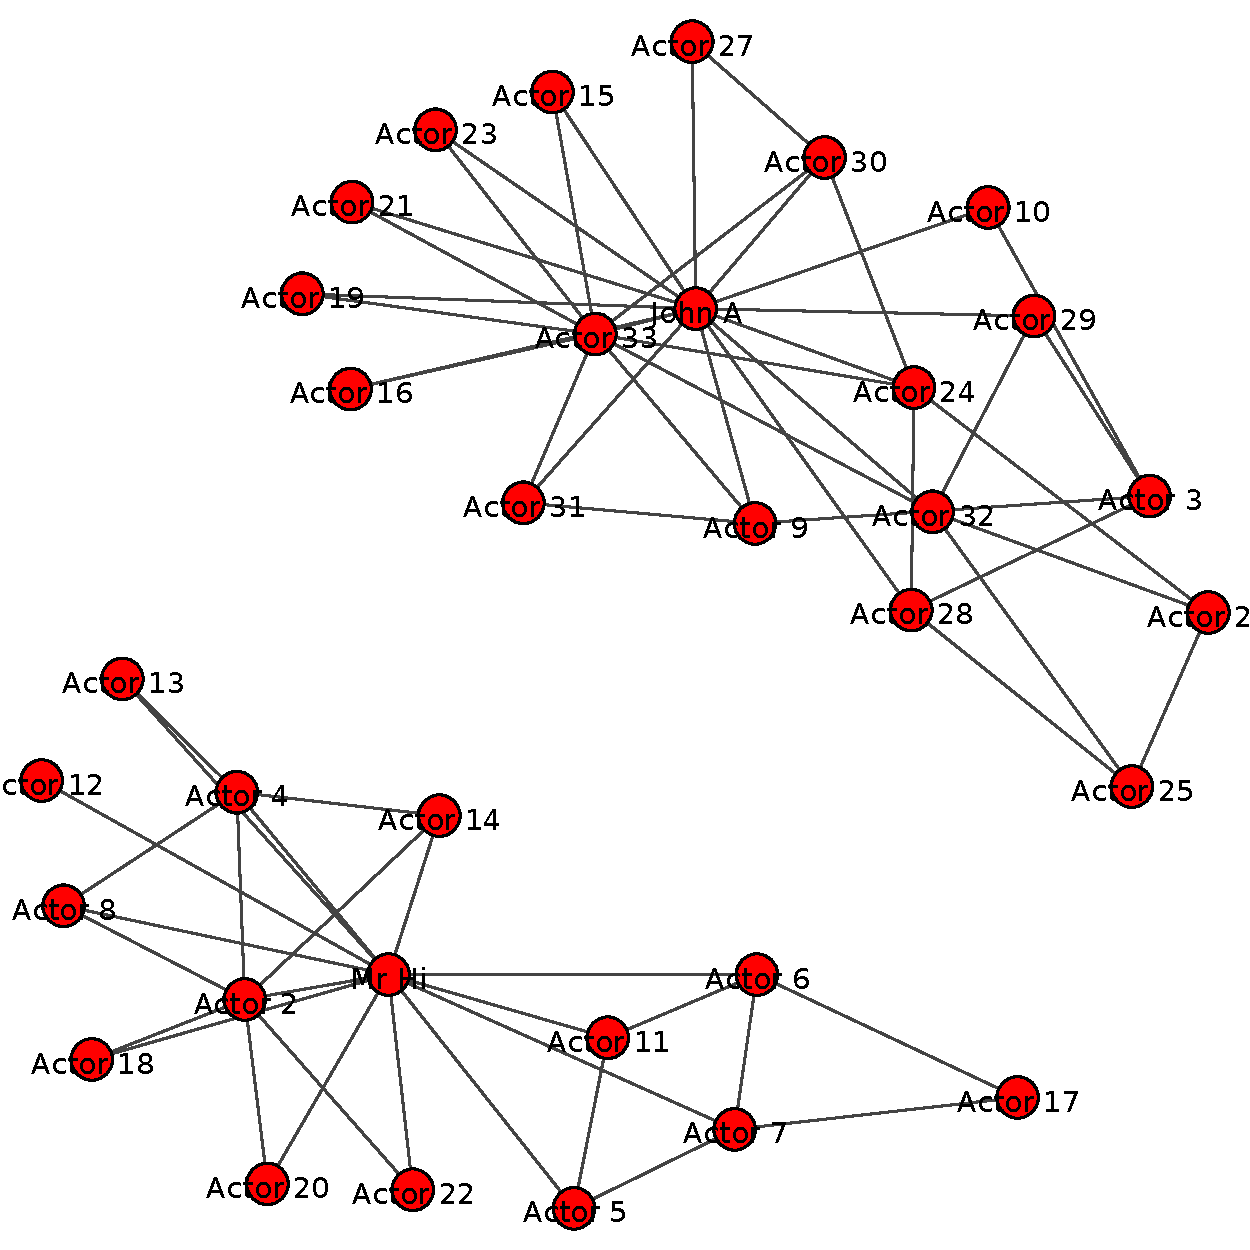
\includegraphics[scale=0.7]{../Q1/graph2.pdf}
\centering
\caption{Graph after split}
\label{fig:Graph after split}
\end{figure}
\newpage

%-----------------------End Question 1----------------------------

%------------------------------------------------------------------
%Question 2 
%------------------------------------------------------------------
\section{Question 2: Karate group split into 3, 4, and 5}
We know that the karate club has been split into 2 groups but assume that there were many arguments in the group and it has split up into a numbers of 3, 4, and 5.
%-----------------------Approach----------------------------------
\subsection{Approach}
Approch to solve the problem is same as question 1 the only difference is  changing the loop condition or writing a bunch of conditional statements.
%-----------------------Source Code---------------------------
\subsection{Source Code}
\subsubsection{karateClubGraphSplit.py}
\lstinputlisting[breaklines=True,language=Python]{../Q2/karateClubGraphSplit.py}
\newpage
%-----------------------Input Section---------------------------
\subsection{Input}
\subsubsection{karate.GraphML}
\lstinputlisting[breaklines=True]{../Q2/karateGraphMLForDoc.txt}
\newpage
%-----------------------Output Section---------------------------
\subsection{Output Files}
\subsubsection{Intial-graph}
Figure~\ref{fig:Initial graph} is the initial graph. According to the requirement the graph can be split into any number of groups just by changing a looping condition in the mathematical model.  Figure~\ref{Initial graph split into 3 groups}, has three clusters, Figure~\ref{Initial graph split into 4 groups} has four clusters, Figure~\ref{Initial graph split into 5 groups} has four clusters formed after splitting the graph with  one cluster.
 
\begin{figure}[ht]
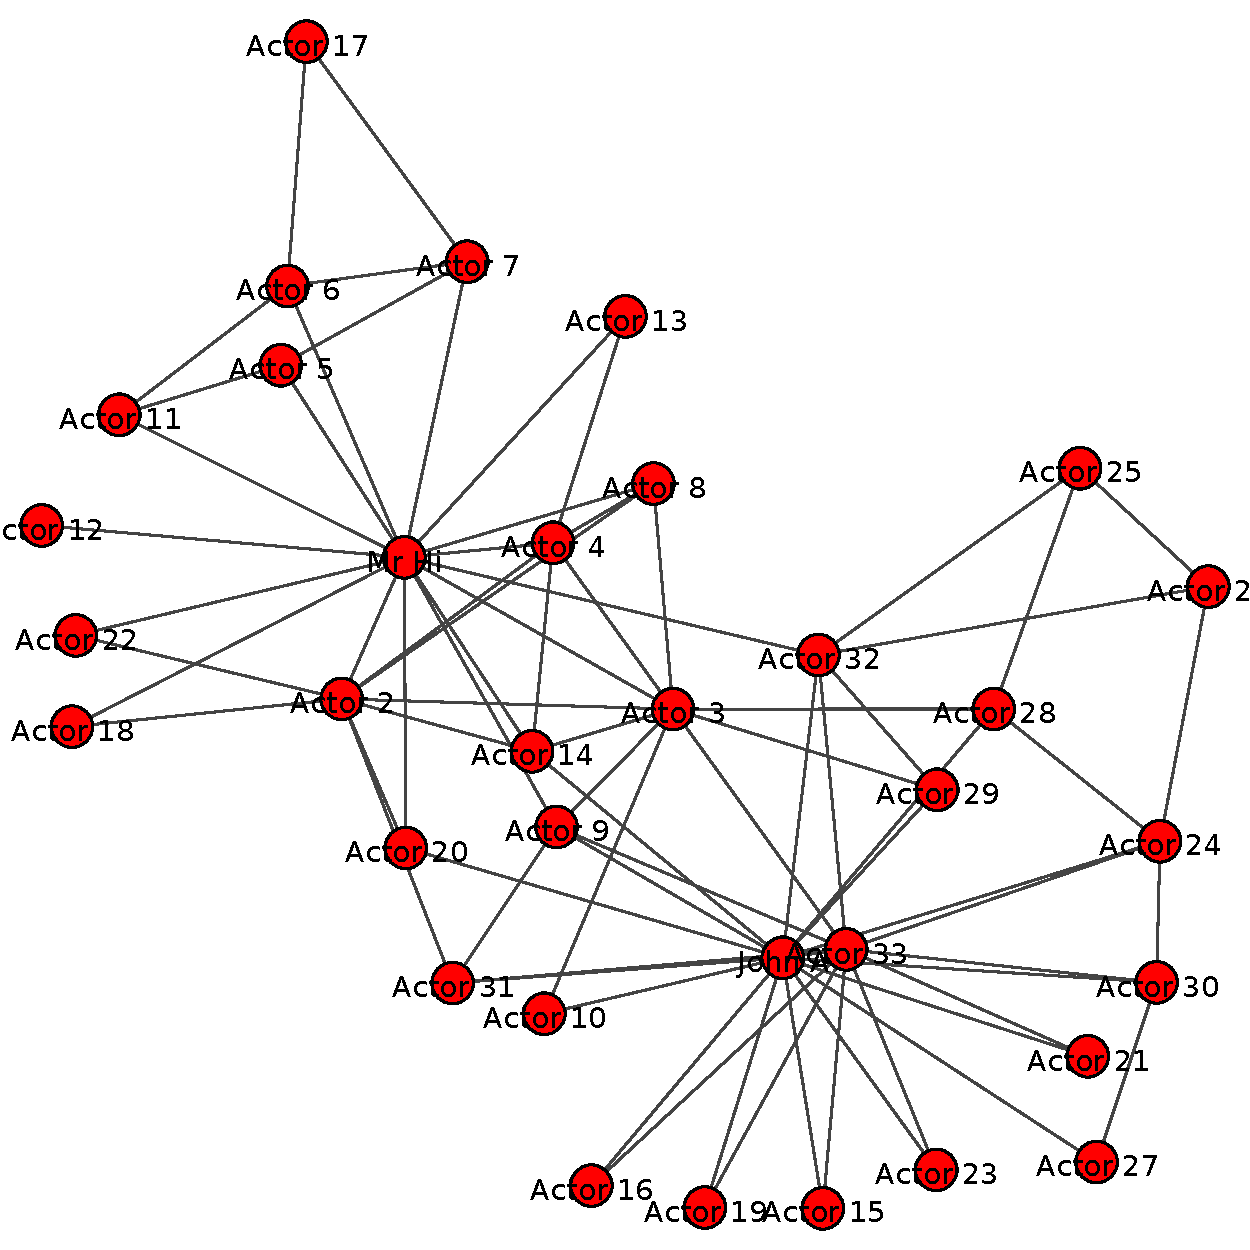
\includegraphics[scale=0.7]{../Q2/graph3.pdf}
\centering
\caption{Initial-graph}
\label{fig:Initial graph}
\end{figure}
\newpage

\subsubsection{Graph after the split}
\begin{figure}[ht]
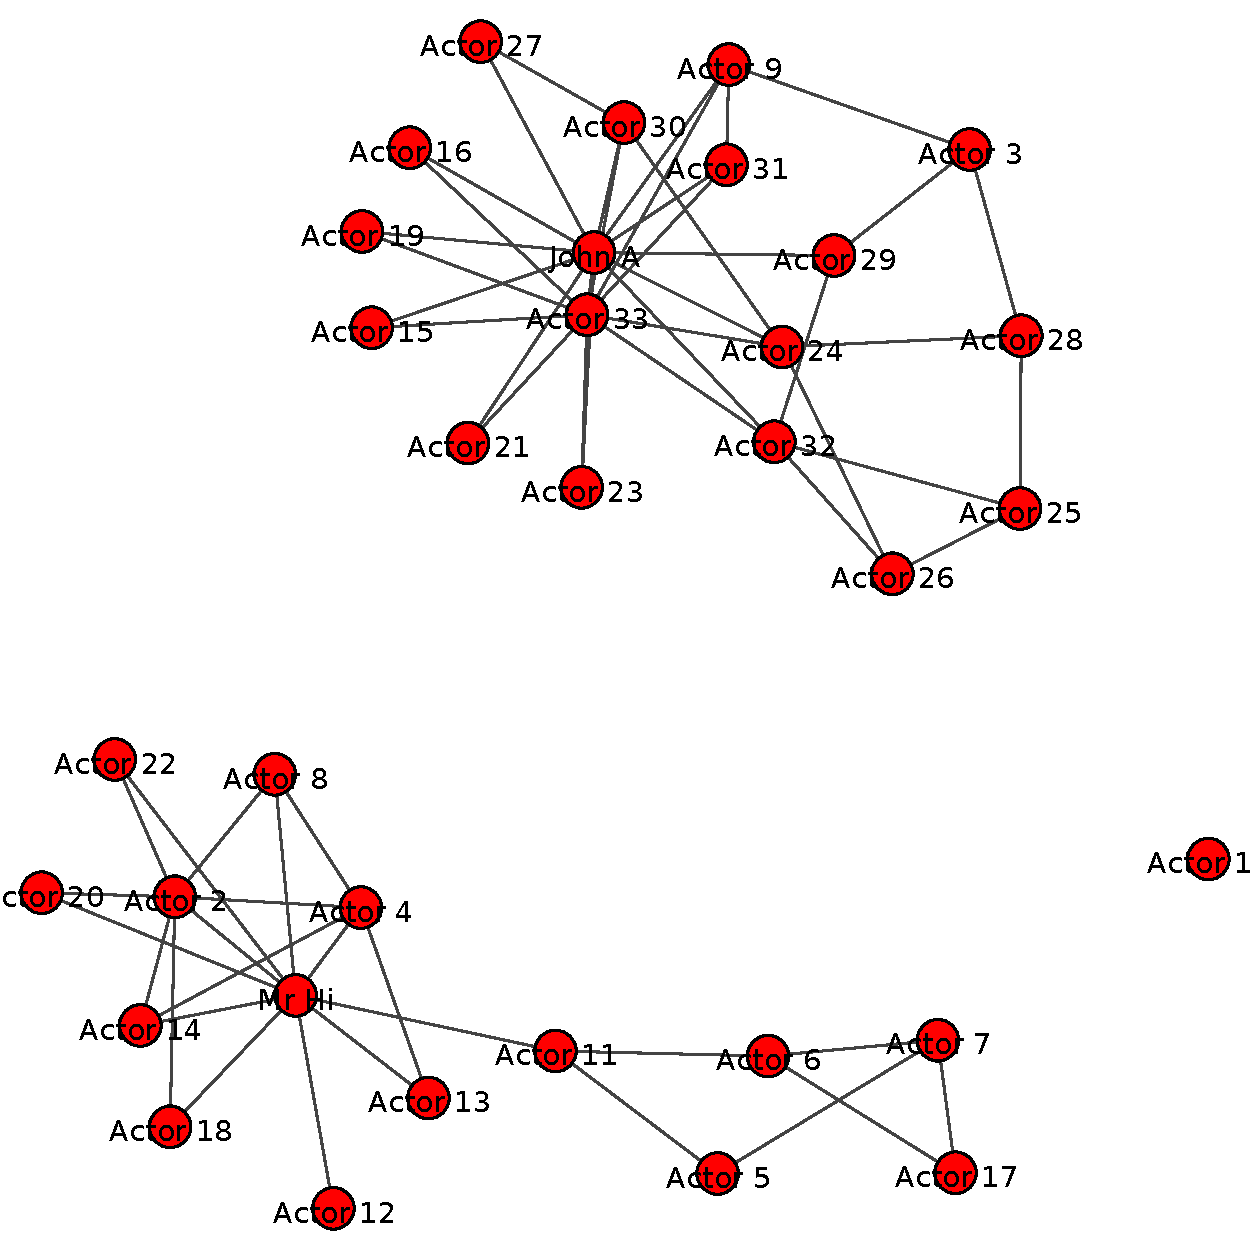
\includegraphics[scale=0.7]{../Q2/graph4.pdf}
\centering
\caption{Initial graph split into 3 groups}
\label{Initial graph split into 3 groups}
\end{figure}
\newpage

\begin{figure}[ht]
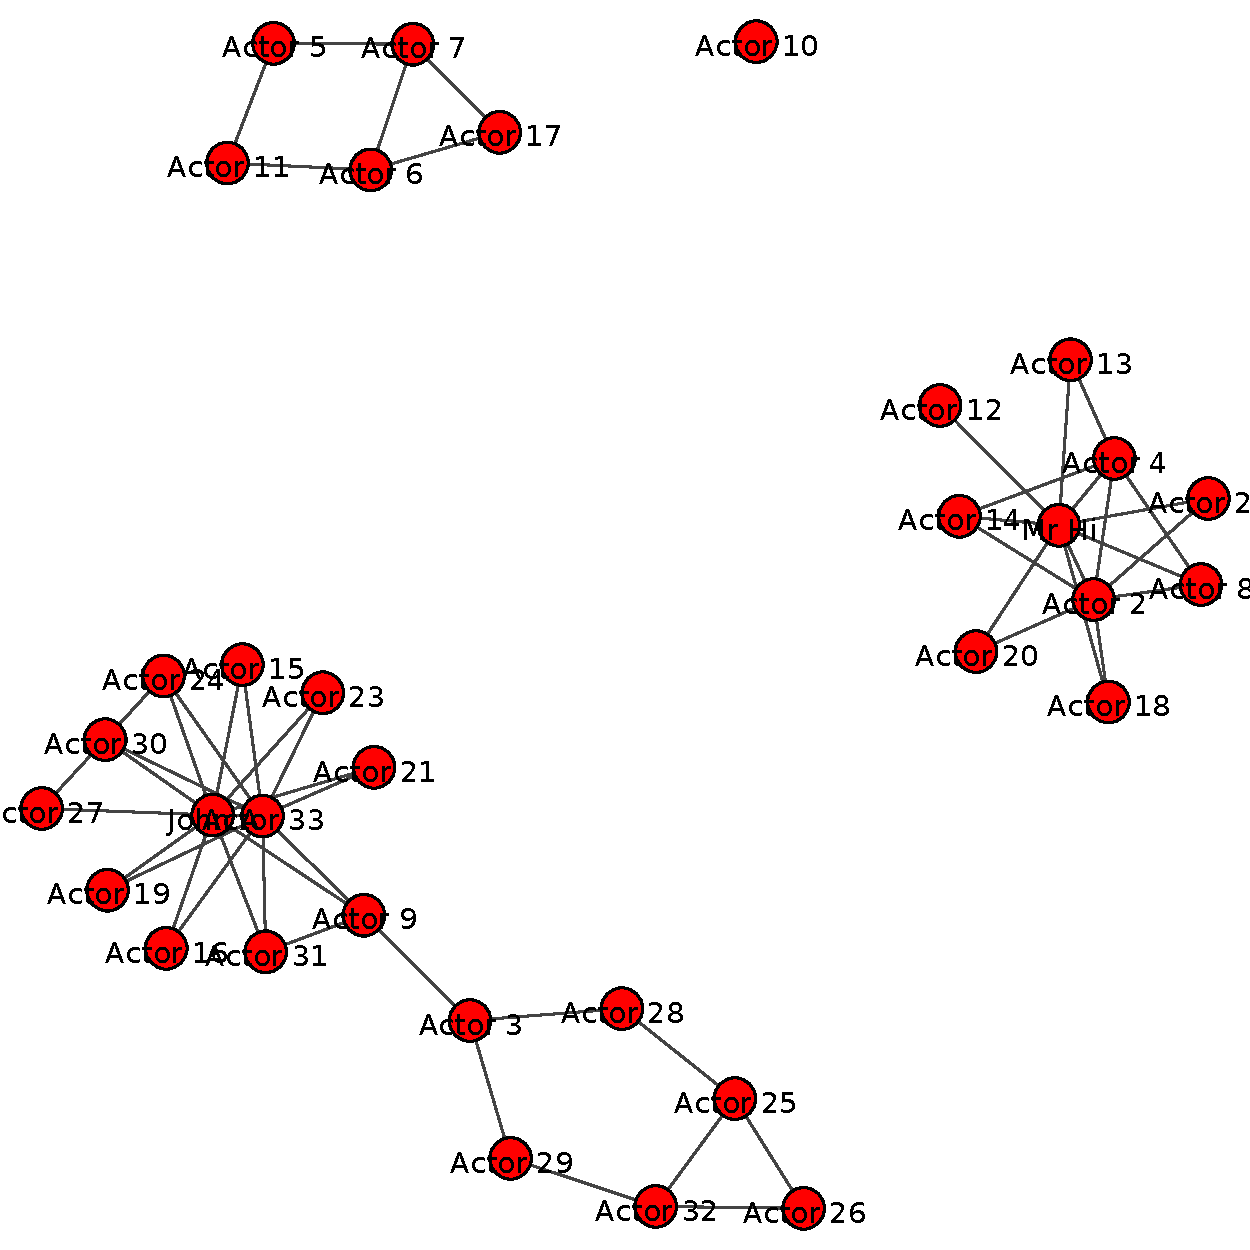
\includegraphics[scale=0.7]{../Q2/graph5.pdf}
\centering
\caption{Initial graph split into 4 groups}
\label{Initial graph split into 4 groups}
\end{figure}
\newpage

\begin{figure}[ht]
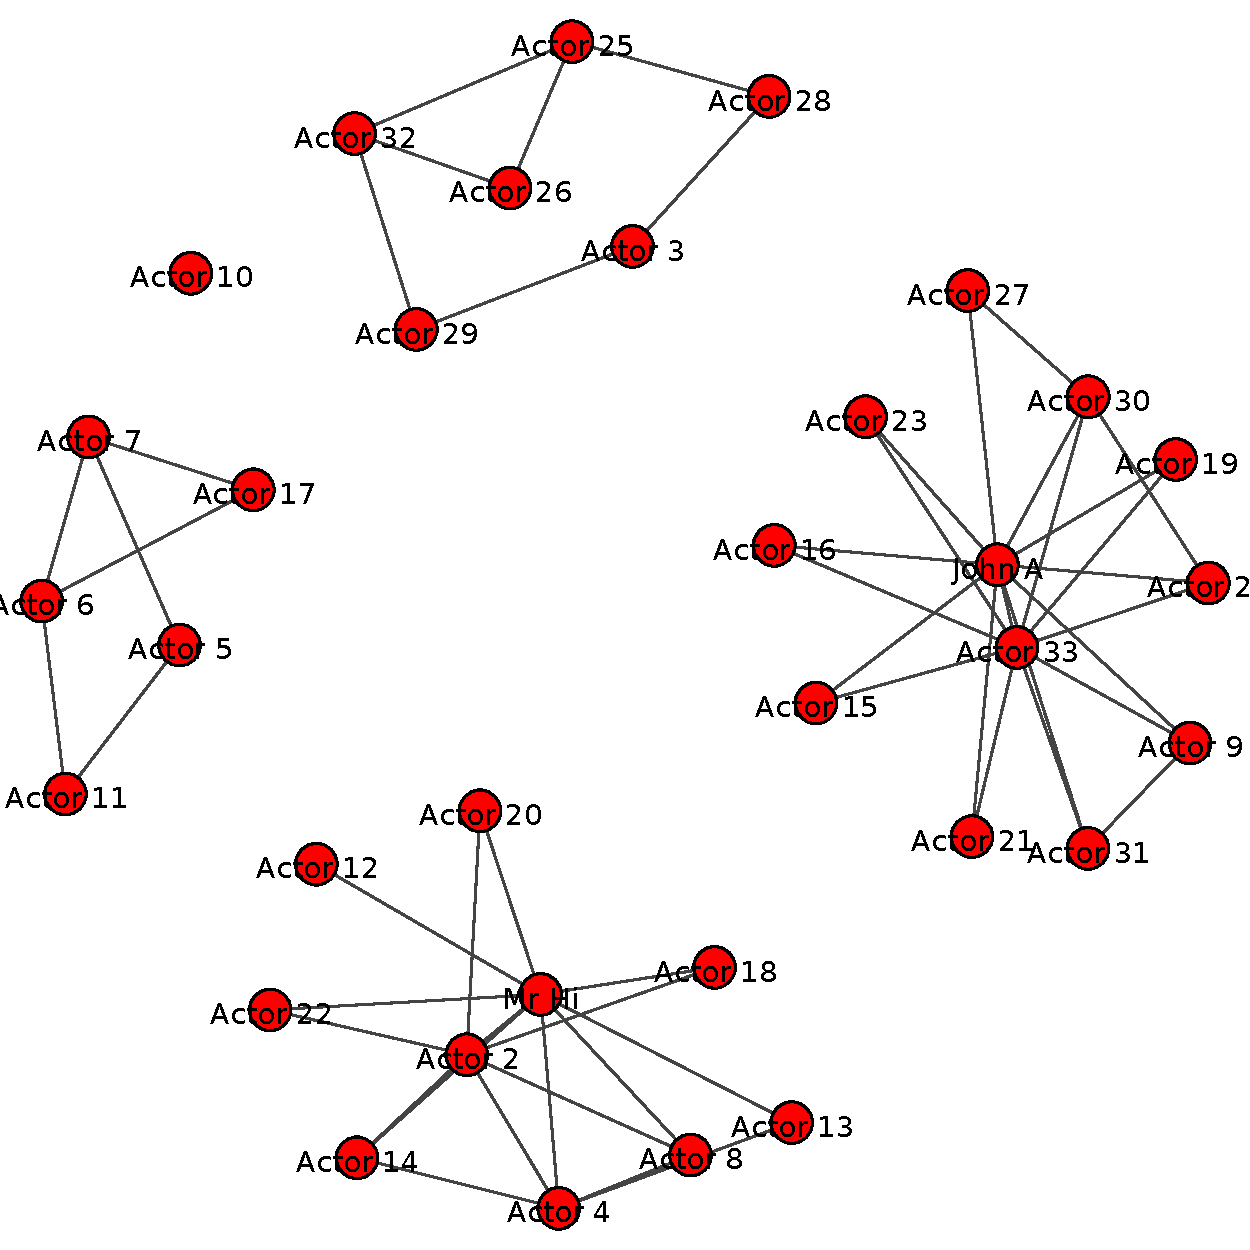
\includegraphics[scale=0.7]{../Q2/graph6.pdf}
\centering
\caption{Initial graph split into 5 groups}
\label{Initial graph split into 5 groups}
\end{figure}
\newpage

\section{Conclusions}
The dispute in the karate club splits the club into two. There are 60 people in the club but we represent a graph with 33 people who are friends and meet outside the club. So, now we know that the club has split into two we try to create a mathematical model which can split the given social network graph into groups in order to achieve this we use Girvan-Newman Algorithm and split the graph and check whether the graphs we obtain match the reality.\\*

When we observe the results from the reality to predicted results they are almost similar except one person. So, the results are not 100\% true but the prediction almost resembles the reality with 96\% (this is value is detremined by using the accuracy formula) similarity. So, the mathematical model best represents the reality from all the above observation. For a real world social network if you want to predict the number of groups in a network this model can be predict the result well.\\*

Hence, we can prove that split results of a group can be predicted by weighted graph using mathematical model.

\newpage
%------------------------------------------------------------------
%Bibilography
%------------------------------------------------------------------
\bibliographystyle{plain}
\bibliography{A6_report}
\cite{*}
\end{document}